\pdfoutput=1
\documentclass[11pt]{article}
\usepackage[T1]{fontenc}
\usepackage[margin=1in]{geometry}
\usepackage{amsmath,amssymb,amsthm,booktabs,array}
\usepackage[shortlabels]{enumitem}
\usepackage[hidelinks]{hyperref}
\usepackage{tikz}
\usetikzlibrary{calc}

\setlist{itemsep=1pt,topsep=3pt}

\newtheorem{theorem}{Theorem}[section]
\newtheorem{lemma}[theorem]{Lemma}
\newtheorem{corollary}[theorem]{Corollary}
\theoremstyle{definition}
\newtheorem{definition}[theorem]{Definition}
\theoremstyle{remark}
\newtheorem{remark}[theorem]{Remark}

\newcommand{\ecc}{\mathrm{ecc}}
\newcommand{\diam}{\mathrm{diam}}
\newcommand{\rad}{\mathrm{rad}}
\newcommand{\DISJ}{\mathrm{DISJ}}
\newcommand{\Ot}{\tilde O}

\title{Quantum Distributed Computation of the Weighted Diameter and Radius of Planar Networks}
\hypersetup{pdftitle={Quantum Distributed Computation of the Weighted Diameter and Radius of Planar Networks},pdfauthor={Sebastian Senge}}
\author{Sebastian Senge\\ Independent Researcher}
\date{}

\begin{document}
\maketitle

\begin{abstract}
We study the exact weighted diameter and radius of planar networks in the CONGEST model. Classically, the weighted diameter of a planar network needs $\Omega(n/\log n)$ rounds already when the hop-diameter is $D = 3$, although the unweighted diameter of planar networks can be computed in a number of rounds polynomial in $D$ and $\log n$. We show that quantum communication reduces the complexity to about $\sqrt n$:
\begin{itemize}[leftmargin=1.5em]
\item There is a Quantum CONGEST algorithm that computes the weighted diameter and the weighted radius of an $n$-node planar network of hop-diameter $D$ exactly in $\Ot(D^2+\sqrt n \cdot D)$ rounds.
\item Every Quantum CONGEST algorithm for the weighted diameter or radius of planar networks needs $\Omega(\sqrt n/\log n)$ rounds, for every hop-diameter $D$ from a small constant up to $n/2$.
\item Every classical CONGEST algorithm for the weighted radius of planar networks needs $\Omega(n/\log n)$ rounds, in the same range of $D$.
\end{itemize}
So for $D$ polylogarithmic in $n$ both problems take $\tilde\Theta(\sqrt n)$ rounds with quantum communication and $\tilde\Theta(n)$ rounds without it. On general networks, a $(3/2-\varepsilon)$-approximation of either quantity already needs $\tilde\Omega(n^{2/3})$ quantum rounds at logarithmic hop-diameter, so planarity makes the exact problems easier for quantum algorithms. The path weights of both lower-bound networks are checked in Lean~4.
\end{abstract}

\section{Introduction}

In the CONGEST model~\cite{Pel00}, the nodes of a network $G=(V,E)$ with $n$ nodes communicate in synchronous rounds, and in each round every node sends a message of $O(\log n)$ bits over each incident edge. The hop-diameter $D$ of $G$ is a lower bound on the number of rounds for every global problem. Distance problems are among the most studied problems in this model. With edge weights, the eccentricity $\ecc(v)$ of a node $v$ is its largest weighted distance to another node, the \emph{diameter} is the largest eccentricity and the \emph{radius} the smallest.

On general networks, computing the diameter exactly takes $\tilde\Theta(n)$ rounds, even without weights and with constant $D$~\cite{FHW12,ACHK16,HW12}, and an $\Ot(n)$ upper bound for the weighted case follows from exact all-pairs shortest paths~\cite{BN19}. In the Quantum CONGEST model, where messages consist of $O(\log n)$ qubits, the unweighted diameter takes $\Ot(\sqrt{nD})$ rounds; $\tilde\Omega(\sqrt n)$ rounds are needed, and $\tilde\Omega(\sqrt{nD})$ rounds when every node has only polylogarithmic quantum memory~\cite{LM18}. With weights, quantum communication helps much less on general networks: a $(3/2-\varepsilon)$-approximation of the weighted diameter or radius needs $\tilde\Omega(n^{2/3})$ quantum rounds even when $D = \Theta(\log n)$, and a $(1+o(1))$-approximation is possible in $\Ot(\min(n^{9/10}D^{3/10}, n))$ rounds~\cite{WY22}. Almost linear quantum lower bounds are also known for computing all eccentricities and all-pairs shortest paths~\cite{WWY22}.

Planar networks behave differently. The unweighted diameter of a planar network can be computed in $\Ot(D^5)$ rounds, and with weights, exact distance labels of $\Ot(D)$ bits can be computed in $\Ot(D^2)$ rounds, after which the distances from any single source follow in $\Ot(D)$ rounds~\cite{LP19}. For the weighted diameter, however, it was shown in~\cite{ACK20} that $\Omega(n/\log n)$ rounds are needed on planar networks of constant hop-diameter. The exact weighted problems on planar networks are thus as hard as on general networks for classical algorithms, while their single-source version is easy.

\paragraph{Contributions.} We show that this gap closes almost completely with quantum communication. Throughout, weights are nonnegative integers bounded by a polynomial in $n$.

\begin{theorem}\label{thm:upper}
There is a Quantum CONGEST algorithm that computes the weighted diameter of an $n$-node planar network of hop-diameter $D$ exactly in $\Ot(D^2+\sqrt n \cdot D)$ rounds, with probability at least $2/3$. The same holds for the weighted radius.
\end{theorem}

\begin{theorem}\label{thm:qlower}
Let $3\le D\le n/2$ for the diameter and $5\le D\le n/2$ for the radius. Every Quantum CONGEST algorithm that, with probability at least $2/3$, computes the weighted diameter, or the weighted radius, of $n$-node planar networks of hop-diameter $D$ takes $\Omega(\sqrt n/\log n)$ rounds.
\end{theorem}

\begin{theorem}\label{thm:clower}
Every classical CONGEST algorithm that, with probability at least $2/3$, computes the weighted radius of $n$-node planar networks of hop-diameter $D$, for $5\le D\le n/2$, takes $\Omega(n/\log n)$ rounds.
\end{theorem}

For the diameter, the classical counterpart of Theorem~\ref{thm:clower} is~\cite[Theorem~9]{ACK20}, with $D=3$ in its proof (Section~3 there), and the padding of Lemma~\ref{lem:pad} extends it to $3\le D\le n/2$. Table~\ref{tab:results} compares the bounds. For $D$ polylogarithmic in $n$, Theorems~\ref{thm:upper} and~\ref{thm:qlower} determine the quantum complexity of both problems up to polylogarithmic factors, and it lies quadratically below the classical complexity.

\begin{table}[h]
\centering
\footnotesize
\renewcommand{\arraystretch}{1.25}
\begin{tabular}{@{}p{2.3cm}p{5.4cm}p{6.6cm}@{}}
\toprule
& Classical CONGEST & Quantum CONGEST\\
\midrule
Upper bound & $\Ot(n)$~\cite{BN19} & $\mathbf{\Ot(D^2+\sqrt n\cdot D)}$ (Theorem~\ref{thm:upper}); before: $\Ot(n)$\\
Lower bound, diameter & $\Omega(n/\log n)$, $D=3$~\cite{ACK20}; $3\le D\le n/2$ (Lemma~\ref{lem:pad}) & $\mathbf{\Omega(\sqrt n/\log n)}$, $3\le D\le n/2$ (Theorem~\ref{thm:qlower})\\
Lower bound, radius & $\mathbf{\Omega(n/\log n)}$, $5\le D\le n/2$ (Theorem~\ref{thm:clower}) & $\mathbf{\Omega(\sqrt n/\log n)}$, $5\le D\le n/2$ (Theorem~\ref{thm:qlower})\\
\bottomrule
\end{tabular}
\caption{Exact weighted diameter and radius of $n$-node planar networks of hop-diameter $D$. On general networks, a $(3/2-\varepsilon)$-approximation needs $\tilde\Omega(n^{2/3})$ quantum rounds for $D=\Theta(\log n)$~\cite{WY22}.}
\label{tab:results}
\end{table}

\paragraph{Techniques.} The upper bound runs the distributed quantum optimization of~\cite{LM18} over the $n$ possible sources. The evaluation must act on a superposition of sources, so it has to be a reversible procedure. We first compute the exact distance labels of~\cite{LP19} once, classically, in $\Ot(D^2)$ rounds. After that, the eccentricity of a source $s$ is a deterministic function of the label of $s$ and the labels of the other nodes: routing the label of $s$ to all nodes and taking a maximum takes $\Ot(D)$ rounds, and this procedure can be run reversibly in superposition. More generally, any randomized exact single-source shortest path algorithm with $T$ rounds gives $\Ot(\sqrt n\,(T+D))$ rounds, by fixing its random bits once for all sources (Remark~\ref{rem:directed}); with the directed algorithm of~\cite{Sen26}, which takes the rotation lists of a planar embedding as input, this gives $\Ot(\sqrt n\cdot D)$ rounds for directed networks.

The lower bounds use the planar network of~\cite{ACK20}, in which the cut between the two players consists of two edges. A simulation in the style of~\cite{LM18} turns a Quantum CONGEST algorithm of $T$ rounds into a two-party protocol with $O(T\log n)$ qubits of communication, and the quantum lower bound of $\Omega(\sqrt k)$ for disjointness of $k$-bit strings~\cite{Raz03} gives Theorem~\ref{thm:qlower} for the diameter. For the radius we change the weights so that the eccentricity of a coordinate node is small exactly when both input bits are $1$, and we attach a leaf to each of the four hubs. The leaves make every hub a poor centre without changing the eccentricities of the coordinate nodes. Finally, a path of weight-$0$ edges at one hub raises the hop-diameter to any value up to $n/2$ without changing the diameter or the radius.

\paragraph{Formal verification.} All path weights used in the analysis of the two lower-bound networks are checked in Lean~4 with Mathlib (Section~\ref{sec:checks}). The distributed algorithms, the cited theorems and the reductions are proved on paper only. A script additionally computes all eccentricities of both networks, with and without padding, for small inputs and checks planarity, the hop-diameters and the cuts.

\paragraph{Organization.} Section~\ref{sec:prelim} recalls the model and the cited tools. Section~\ref{sec:upper} proves Theorem~\ref{thm:upper}, Section~\ref{sec:lower} proves Theorems~\ref{thm:qlower} and~\ref{thm:clower}, and Section~\ref{sec:checks} describes the machine checks.

\section{Model and tools}\label{sec:prelim}

\paragraph{Networks.} A network is a connected undirected graph $G=(V,E)$ with $n$ nodes, distinct identifiers from $\{1,\dots,\mathrm{poly}(n)\}$, and edge weights $w\colon E\to\{0,\dots,W\}$ known to the two endpoints of each edge, where $W$ is bounded by a polynomial in $n$ that all nodes know. We write $d(u,v)$ for the weighted distance, $\ecc(v)=\max_u d(v,u)$, $\diam(G)=\max_v \ecc(v)$ and $\rad(G)=\min_v\ecc(v)$. The hop-diameter $D$ is the diameter of $G$ without weights. A network is planar if its graph is.

\paragraph{CONGEST and Quantum CONGEST.} In the CONGEST model, computation proceeds in synchronous rounds; in each round every node performs local computation and sends a message of $O(\log n)$ bits over each incident edge. Nodes have unbounded local memory and private random bits. In the Quantum CONGEST model~\cite{EKNP14,LM18}, nodes hold quantum registers, perform arbitrary local quantum operations, and send $O(\log n)$ qubits over each edge per round; initially they share no entanglement. An algorithm computes a quantity if at the end some node outputs it; one more $O(D)$ rounds make it known to all nodes.

\paragraph{Distributed quantum optimization.} Let $X$ be a finite set and $f\colon X\to\mathbb{Z}$. Following~\cite{LM18}, the procedure \emph{Setup} prepares $|X|^{-1/2}\sum_{x\in X}|x\rangle$ in a register of a leader node, and the procedure \emph{Evaluation} maps $|x\rangle|0\rangle\mapsto|x\rangle|f(x)\rangle$, where both registers are held by the leader and all other registers of the network start and end in a fixed state.

\begin{theorem}[{\cite[Theorem~7]{LM18}}]\label{thm:qopt}
Suppose that an initialization can be done in $T_0$ rounds and that Setup, Evaluation and their inverses can be implemented in $T$ rounds in the Quantum CONGEST model. Let $\varepsilon>0$ be a lower bound on the fraction of elements $x\in X$ at which $f$ is maximum. Then for every $\delta>0$ the leader finds such an element with probability at least $1-\delta$ in $T_0 + O(\log(1/\delta)/\sqrt\varepsilon)\cdot T$ rounds.
\end{theorem}

Minimization is the same with $-f$ in place of $f$.

\paragraph{Shortest paths in planar networks.}

A \emph{distance labelling} assigns to every node $v$ a bit string $L(v)$ such that $d(u,v)$ is a fixed function of $L(u)$ and $L(v)$.

\begin{theorem}[{\cite[Lemmas~5.1 and~5.2]{LP19}}]\label{thm:sssp}
There is a randomized CONGEST algorithm that computes, in an $n$-node planar network of hop-diameter $D$ with largest weight $W$, an exact distance labelling with labels of $O(D\log n\log W)$ bits, every node learning its own label, in $\Ot(D^2\log W)$ rounds with high probability.
\end{theorem}

The exact single-source shortest path algorithm of~\cite[Theorem~1.6 and Lemma~5.3]{LP19} sends the label of the source to all nodes after this step. Since $W=\mathrm{poly}(n)$, the labels have $\Ot(D)$ bits and the labelling takes $\Ot(D^2)$ rounds. We use it with failure probability at most $1/n$; the nodes stop it after a fixed number of rounds, computed from $n$, the polynomial bound on $W$ and a $2$-approximation of $D$, that it respects with this probability.

\paragraph{Disjointness.} In the two-party problem $\DISJ_k$, Alice holds $A\in\{0,1\}^k$, Bob holds $B\in\{0,1\}^k$, and they must decide whether $A_i=B_i=1$ for some $i$.

\begin{theorem}\label{thm:disj}
Every randomized protocol for $\DISJ_k$ with error at most $1/3$ communicates $\Omega(k)$ bits~\cite{KS92,Raz92}, and every quantum protocol with error at most $1/3$ communicates $\Omega(\sqrt k)$ qubits~\cite{Raz03}.
\end{theorem}

\paragraph{Simulation.} The following is the standard reduction from two-party communication, in the form used in~\cite[Theorem~10]{LM18}.

\begin{lemma}\label{lem:sim}
Let $V = V_A\sqcup V_B$ be a fixed set of $n$ nodes with fixed identifiers, and let $G(A,B)$ be networks on $V$ with a fixed edge set, in which the weights of edges inside $V_A$ depend only on $A$, the weights of edges inside $V_B$ depend only on $B$, and exactly $b$ edges join $V_A$ and $V_B$, with fixed weights. If a Quantum CONGEST algorithm of $T$ rounds computes, with probability at least $2/3$, a quantity from which $\DISJ_k(A,B)$ can be read off, then $\DISJ_k$ has a quantum protocol with error at most $1/3$ and $O(Tb\log n)$ qubits of communication. The same holds for classical algorithms and bits.
\end{lemma}

\begin{proof}
Alice simulates all nodes of $V_A$ and Bob all nodes of $V_B$; each knows the edges and weights at its own nodes. Messages over edges inside one side are simulated locally. In each round, Alice sends to Bob the qubits that her nodes send over the $b$ crossing edges, and Bob does the same; these are $O(b\log n)$ qubits per round. After $T$ rounds, the player who simulates the output node measures, reads off $\DISJ_k(A,B)$ and sends one bit to the other player. Since the joint state of the simulation equals the state of the network at every round, the protocol errs with probability at most $1/3$. With classical messages the argument is the same.
\end{proof}

\section{Upper bound}\label{sec:upper}

Let $G$ be an $n$-node planar network of hop-diameter $D$.

\paragraph{Initialization.} In $\Ot(D)$ rounds the nodes elect a leader, build a BFS tree rooted at the leader, compute a value $D'$ with $D\le D'\le 2D$, and replace their identifiers by the numbers $1,\dots,n$ (from subtree sizes, assigned top-down along the tree). Then they compute the labelling of Theorem~\ref{thm:sssp} in $\Ot(D^2)$ rounds. With probability at least $1-1/n$ all labels are correct; from now on we assume this, and the rest of the algorithm is deterministic. All labels are padded to the same length $\lambda=\Ot(D)$ bits, which every node can compute.

Let $N=2^{\lceil\log_2 n\rceil}$ and $X=\{1,\dots,N\}$, and let $f(s)=\ecc(s)$ for $s\le n$ and $f(s)=-1$ for $s>n$. Setup, the uniform superposition over $X$, is a local operation of the leader, and the fraction of maximizers of $f$ is at least $1/N\ge 1/(2n)$.

\begin{lemma}[Evaluation]\label{lem:eval}
After the initialization, Evaluation and its inverse for $f$ can be implemented in $\Ot(D)$ rounds of Quantum CONGEST.
\end{lemma}

\begin{proof}
All steps act on computational basis states and are made reversible by keeping every intermediate value in fresh registers; message qubits are copies made with CNOT gates.
\begin{enumerate}[1.]
\item The leader sends a copy of $s$ down the BFS tree, in $O(D)$ rounds. Every node keeps its copy and checks whether $s$ is its own number.
\item The label of $s$ is moved to the leader. Every node $v$ holds a register of $\lambda$ bits that contains $L(v)$ if $v=s$ and zeros otherwise. Bottom-up along the tree, every node sends the bitwise XOR of its register and the strings received from its children, in pieces of $O(\log n)$ bits and pipelined. Since exactly one register is nonzero, the leader receives $L(s)$ after $O(D+\lambda/\log n)=\Ot(D)$ rounds. For $s>n$, which the leader decides by comparing $s$ with $n$, the output is $-1$ and the steps below are skipped under this control.
\item The leader sends $L(s)$ down the tree, pipelined, in $\Ot(D)$ rounds.
\item Every node $v$ computes $d(s,v)$ from $L(s)$ and $L(v)$ locally. The maximum over all nodes is computed bottom-up along the tree, in $O(D)$ rounds, and the leader copies it into the output register.
\item Steps 4 to 1 are undone in reverse order, which returns all registers except the input and the output to their initial state.
\end{enumerate}
The total is $\Ot(D)$ rounds. The inverse is the same circuit run backwards.
\end{proof}

\begin{proof}[Proof of Theorem~\ref{thm:upper}]
The initialization takes $T_0=\Ot(D^2)$ rounds and fails with probability at most $1/n$. Given correct labels, Theorem~\ref{thm:qopt} with $\varepsilon=1/(2n)$, $\delta=1/6$ and Lemma~\ref{lem:eval} finds a source $s^*$ of maximum eccentricity in $\Ot(D^2)+O(\sqrt n)\cdot\Ot(D)=\Ot(D^2+\sqrt n\cdot D)$ rounds, and one more evaluation gives $\diam(G)=\ecc(s^*)$. The total failure probability is at most $1/6+1/n\le 1/3$ for $n\ge 6$. For the radius, run the same algorithm with $f(s)=-\ecc(s)$ for $s\le n$ and $f(s)=-nW-1$ for $s>n$.
\end{proof}

\begin{remark}\label{rem:directed}
Let $P$ be any randomized CONGEST algorithm that computes exact distances from a given source in $T$ rounds with failure probability at most $n^{-2}$. If every node draws its random bits for $P$ once, before the search, then by the union bound these bits are good for all $n$ sources at once with probability at least $1-1/n$. With these bits fixed, $P$ followed by a maximum over the tree is a deterministic procedure from $s$ to $\ecc(s)$, and running it reversibly as in Lemma~\ref{lem:eval} gives $\Ot(\sqrt n\,(T+D))$ rounds. In~\cite{Sen26}, exact single-source shortest paths in directed planar networks with nonnegative weights are computed in $\Ot(D)$ rounds, given the rotation lists of a planar embedding, assuming several cited results that are listed there as hypotheses. Under the same assumptions, this gives $\Ot(\sqrt n\cdot D)$ rounds for the diameter and radius of directed planar networks (with distances in the directed sense, and communication over the underlying undirected network).
\end{remark}

\section{Lower bounds}\label{sec:lower}

\subsection{The network}

For $k\ge 1$, an integer $M\ge 2$ and bits $\alpha_1,\dots,\alpha_k,\beta_1,\dots,\beta_k\in\{0,1\}$, let $N=N_M(\alpha,\beta)$ be the following network, which is the network in the proof of~\cite[Theorem~9]{ACK20} with general weights; see Figure~\ref{fig:network}. Its nodes are the \emph{coordinate nodes} $a_1,\dots,a_k$ and $b_1,\dots,b_k$ and the \emph{hubs} $\ell, r, \ell', r'$. Each $a_i$ is joined to $\ell$ and to $r$, each $b_j$ to $\ell'$ and to $r'$, and there are the two \emph{crossing edges} $\ell\ell'$ and $rr'$. The weights are
\[
w(a_i\ell)=iM+\alpha_i,\quad w(a_ir)=(k+1-i)M+\alpha_i,\quad w(b_j\ell')=(k+1-j)M+\beta_j,\quad w(b_jr')=jM+\beta_j,
\]
and $w(\ell\ell')=w(rr')=M$. Alice's side is $V_A=\{a_1,\dots,a_k,\ell,r\}$, and Bob's side is $V_B=\{b_1,\dots,b_k,\ell',r'\}$.

\begin{figure}[t]
\centering
% The lower-bound network for k = 3. Dashed: the leaves of the radius network.
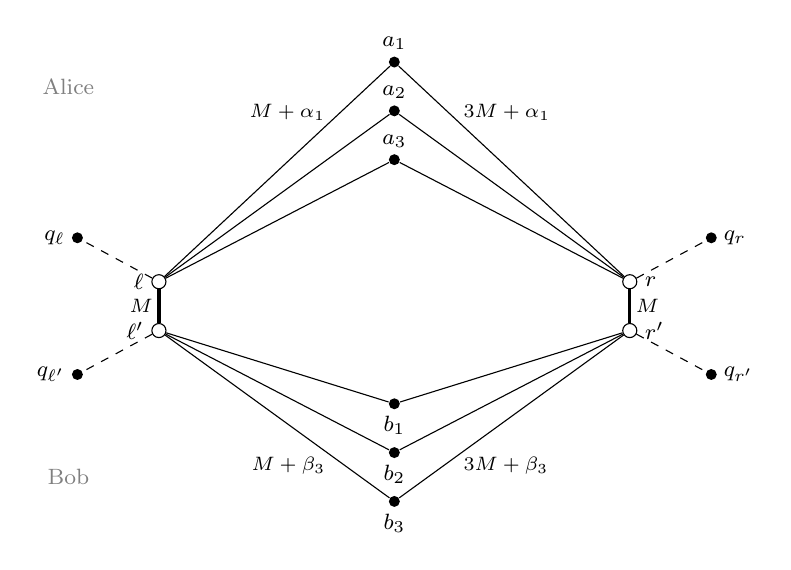
\begin{tikzpicture}[x=1.15cm,y=0.62cm,
  v/.style={circle,fill=black,inner sep=1.4pt},
  hub/.style={circle,draw,fill=white,inner sep=1.8pt},
  lab/.style={font=\footnotesize},
  wt/.style={font=\scriptsize,fill=white,inner sep=1pt}]
  % Alice: a_1 at the top
  \foreach \i/\y in {1/6,2/5,3/4} {\node[v] (a\i) at (0,\y) {};}
  \foreach \i/\y in {1/-1,2/-2,3/-3} {\node[v] (b\i) at (0,\y) {};}
  \node[hub] (l) at (-2.6,1.5) {}; \node[hub] (r) at (2.6,1.5) {};
  \node[hub] (lp) at (-2.6,0.5) {}; \node[hub] (rp) at (2.6,0.5) {};
  \foreach \i in {1,2,3} {\draw (a\i) -- (l); \draw (a\i) -- (r); \draw (b\i) -- (lp); \draw (b\i) -- (rp);}
  \draw[very thick] (l) -- (lp); \draw[very thick] (r) -- (rp);
  % labels
  \foreach \i in {1,2,3} {\node[lab,above=1pt] at (a\i) {$a_{\i}$}; \node[lab,below=1pt] at (b\i) {$b_{\i}$};}
  \node[lab,left=2pt] at (l) {$\ell$}; \node[lab,right=2pt] at (r) {$r$};
  \node[lab,left=2pt] at (lp) {$\ell'$}; \node[lab,right=2pt] at (rp) {$r'$};
  % weights on the edges at a_1 and b_3
  \node[wt,anchor=south east] at ($(a1)!0.28!(l)$) {$M+\alpha_1$};
  \node[wt,anchor=south west] at ($(a1)!0.28!(r)$) {$3M+\alpha_1$};
  \node[wt,anchor=north east] at ($(b3)!0.28!(lp)$) {$M+\beta_3$};
  \node[wt,anchor=north west] at ($(b3)!0.28!(rp)$) {$3M+\beta_3$};
  \node[wt,left=1pt] at ($(l)!0.5!(lp)$) {$M$};
  \node[wt,right=1pt] at ($(r)!0.5!(rp)$) {$M$};
  % leaves of the radius network
  \foreach \h/\dx/\dy in {l/-0.9/0.9,r/0.9/0.9,lp/-0.9/-0.9,rp/0.9/-0.9} {
    \node[v] (q\h) at ($(\h)+(\dx,\dy)$) {};
    \draw[dashed] (\h) -- (q\h);}
  \node[lab,left=1pt] at (ql) {$q_\ell$}; \node[lab,right=1pt] at (qr) {$q_r$};
  \node[lab,left=1pt] at (qlp) {$q_{\ell'}$}; \node[lab,right=1pt] at (qrp) {$q_{r'}$};
  \node[lab,gray] at (-3.6,5.5) {Alice};
  \node[lab,gray] at (-3.6,-2.5) {Bob};
\end{tikzpicture}

\caption{The network $N_M(\alpha,\beta)$ for $k=3$, with the weights at $a_1$ and $b_3$. The crossing edges $\ell\ell'$ and $rr'$ (thick) are the only edges between Alice's side and Bob's side. The dashed leaves are added for the radius.}
\label{fig:network}
\end{figure}

\begin{lemma}\label{lem:structure}
The network $N$ is planar, has hop-diameter $3$, and exactly two edges join $V_A$ and $V_B$.
\end{lemma}

\begin{proof}
Place $\ell=(-1,0)$, $r=(1,0)$, $\ell'=(-1,-1)$, $r'=(1,-1)$, $a_i=(0,i)$ and $b_j=(0,-1-j)$, and draw all edges as straight segments. The edges joining $\ell$ and $r$ to the nodes $a_i$ lie in the half-planes $x\le 0$ and $x\ge 0$ and in the region $y\ge 0$, the edges joining $\ell'$ and $r'$ to the nodes $b_j$ lie in the same half-planes and in the region $y\le -1$, and the crossing edges are the vertical segments at $x=\pm1$. Segments from a common endpoint meet only there, and segments in different regions meet at most at endpoints, so the drawing is planar. Every coordinate node is adjacent to two hubs, every hub on one side is adjacent to a hub on the other side, and the hubs $\ell, r$ have the common neighbour $a_1$; checking the pairs gives hop-diameter $3$, attained by $a_1$ and $b_1$. The two crossing edges are the only edges between the sides.
\end{proof}

\begin{lemma}[Distances in $N$]\label{lem:dist}
For all $i\ne j$ in $\{1,\dots,k\}$ and every hub $h$:
\begin{enumerate}[(a)]
\item $d(a_i,b_i)=(k+2)M+\alpha_i+\beta_i$;
\item $d(a_i,b_j)$, $d(a_i,a_j)$ and $d(b_i,b_j)$ are at most $(k+1)M+2$;
\item $d(a_i,h)$ and $d(b_i,h)$ are at most $(k+1)M+1$;
\item $d(\ell,r)$ and $d(\ell',r')$ are at most $(k+1)M+2$, $d(\ell,\ell')=d(r,r')=M$, and
\[
(k+2)M\le d(\ell,r'),\,d(r,\ell')\le (k+2)M+2\min(\alpha_1,\beta_1).
\]
\end{enumerate}
\end{lemma}

\begin{proof}
Every edge has weight at least $M$, and every coordinate node has degree $2$, with total weight $(k+1)M+2\alpha_i$ at $a_i$ and $(k+1)M+2\beta_j$ at $b_j$.

(a) The paths $a_i\,\ell\,\ell'\,b_i$ and $a_i\,r\,r'\,b_i$ both weigh $(k+2)M+\alpha_i+\beta_i$. Let $P$ be any simple path from $a_i$ to $b_i$. If no inner node of $P$ is a coordinate node, then the inner nodes of $P$ are hubs, and since the only edges between hubs are the crossing edges, $P$ is one of the two paths above. Otherwise $P$ passes through a coordinate node $x$ and uses both edges at $x$, of total weight at least $(k+1)M$. The first and the last edge of $P$ and one crossing edge are three further edges, so $P$ weighs at least $(k+4)M>(k+2)M+2$.

(b) For $i<j$, the path $a_i\,\ell\,\ell'\,b_j$ weighs $(k+2-(j-i))M+\alpha_i+\beta_j\le(k+1)M+2$; for $i>j$ the path through $r$ and $r'$ is the same. The two paths $a_i\,\ell\,a_j$ and $a_i\,r\,a_j$ weigh $(i+j)M$ and $(2k+2-i-j)M$, plus $\alpha_i+\alpha_j$, and the smaller is at most $(k+1)M+2$. Bob's side is symmetric.

(c) The edges give $d(a_i,\ell)\le kM+1$ and $d(a_i,r)\le kM+1$, and adding a crossing edge gives $d(a_i,\ell')\le(i+1)M+1$ and $d(a_i,r')\le(k+2-i)M+1$, all at most $(k+1)M+1$. Bob's side is symmetric.

(d) The paths $\ell\,a_1\,r$ and $\ell'\,b_1\,r'$ weigh $(k+1)M+2\alpha_1$ and $(k+1)M+2\beta_1$. The paths $\ell\,\ell'\,b_1\,r'$ and $\ell\,a_1\,r\,r'$ weigh $(k+2)M+2\beta_1$ and $(k+2)M+2\alpha_1$, and so do the paths $r\,r'\,b_1\,\ell'$ and $r\,a_1\,\ell\,\ell'$. For the lower bound, a simple path from $\ell$ to $r'$ either uses $\ell\ell'$ and then goes from $\ell'$ to $r'$ through some $b_j$, or goes from $\ell$ to $r$ through some $a_i$ and then uses $rr'$. In both cases it weighs at least $M+(k+1)M$. The pair $r,\ell'$ is symmetric.
\end{proof}

The case analysis of~\cite{ACK20} covers the pairs in (a), (b) and (c); we include the hub pairs in (d) for completeness.

\subsection{Diameter}

\begin{corollary}\label{cor:diam}
Let $M=4$, $\alpha_i=A_i$ and $\beta_j=B_j$. Then $\diam(N)=4(k+2)+2$ if $A_i=B_i=1$ for some $i$, and $\diam(N)\le 4(k+2)+1$ otherwise.
\end{corollary}

\begin{proof}
By Lemma~\ref{lem:dist}, every distance is at most $(k+2)M+2$, and by (a) this value is attained if $A_i=B_i=1$ for some $i$. If there is no such $i$, then (a) gives at most $(k+2)M+1$ for the pairs $a_i,b_i$, (d) gives at most $(k+2)M$ for the hub pairs since $\min(\alpha_1,\beta_1)=0$, and (b), (c), (d) give at most $(k+1)M+2$ for all other pairs.
\end{proof}

\subsection{Radius}

Let $N^\circ=N^\circ_M(\alpha,\beta)$ be the network $N_M(\alpha,\beta)$ with four further nodes $q_\ell,q_r,q_{\ell'},q_{r'}$, where $q_h$ is a leaf joined to the hub $h$ by an edge of weight $3$. The leaves $q_\ell,q_r$ belong to Alice's side and $q_{\ell'},q_{r'}$ to Bob's.

\begin{lemma}\label{lem:radius}
Let $M=5$, $\alpha_i=1-A_i$ and $\beta_j=1-B_j$. The network $N^\circ$ is planar, has hop-diameter $5$ and two crossing edges, and
\[
\rad(N^\circ)=5(k+2)+\min_i\bigl((1-A_i)+(1-B_i)\bigr).
\]
In particular $\rad(N^\circ)=5(k+2)$ if $A_i=B_i=1$ for some $i$, and $\rad(N^\circ)\ge 5(k+2)+1$ otherwise.
\end{lemma}

\begin{proof}
Adding leaves preserves planarity and the cut, and adds at most $2$ to every hop distance; the pair $q_\ell,q_{r'}$ is at hop distance $5$. Since the leaves have degree $1$, distances between nodes of $N$ are the same in $N^\circ$, and $d(x,q_h)=d(x,h)+3$.

For a coordinate node $a_i$, Lemma~\ref{lem:dist}(b) and (c) bound its distance to every coordinate node other than $b_i$ by $(k+1)M+2$, its distance to every hub by $(k+1)M+1$, and its distance to every leaf by $(k+1)M+4<(k+2)M$, as $M=5$. With (a), $\ecc(a_i)=d(a_i,b_i)=(k+2)M+\alpha_i+\beta_i$, and the same holds for $b_i$. For the hub $\ell$, Lemma~\ref{lem:dist}(d) gives $\ecc(\ell)\ge d(\ell,q_{r'})=d(\ell,r')+3\ge(k+2)M+3$, and in the same way $\ecc(r)\ge d(r,q_{\ell'})$, $\ecc(\ell')\ge d(\ell',q_r)$ and $\ecc(r')\ge d(r',q_\ell)$ are at least $(k+2)M+3$. A leaf $q_h$ has $\ecc(q_h)=\ecc(h)+3$. So the minimum eccentricity is attained at a coordinate node, and it is $(k+2)M+\min_i(\alpha_i+\beta_i)$.
\end{proof}

\subsection{Padding}

For $t\ge 0$, let $N_M(\alpha,\beta;t)$ and $N^\circ_M(\alpha,\beta;t)$ arise from $N_M(\alpha,\beta)$ and $N^\circ_M(\alpha,\beta)$ by adding a path $\ell\,p_1\,p_2\cdots p_t$ of new nodes on Alice's side, with edges of weight~$0$, and optionally one more new node $p'_t$ on Alice's side: for $t\ge1$ it is joined by an edge of weight~$0$ to $p_{t-1}$ (to $\ell$ if $t=1$), and for $t=0$ it is joined to $\ell$ by an edge of weight~$0$ and to $r$ by an edge of weight $(k+1)M+2$.

\begin{lemma}\label{lem:pad}
Padding preserves planarity, the cut, the diameter and the radius. The hop-diameter of $N_M(\alpha,\beta;t)$ is $t+3$, and that of $N^\circ_M(\alpha,\beta;t)$ is $\max(5,t+4)$.
\end{lemma}

\begin{proof}
The new nodes form a path or a tree attached at $\ell$, except for $p'_0$, which can be drawn like a further coordinate node $a_0$ above $a_1$. So planarity and the two crossing edges are preserved. Every new node $p$ has $d(x,p)=d(x,\ell)$ for all old nodes $x$, since for $p'_0$ the path through $r$ is no shorter ($d(x,\ell)\le d(x,r)+d(r,\ell)$ and $d(r,\ell)\le(k+1)M+2$ by Lemma~\ref{lem:dist}(d)), and the new nodes are at distance $0$ from each other. The path $\ell\,p'_0\,r$ weighs at least $d(\ell,r)$, so the distances between old nodes do not change, $\ecc(x)$ does not change for old nodes $x$ (since $d(x,p)=d(x,\ell)\le\ecc(x)$), and $\ecc(p)=\ecc(\ell)$. So neither the largest nor the smallest eccentricity changes. In $N$, the node $\ell$ is at hop distance at most $3$ from every node, and exactly $3$ from $r'$; so for $t\ge1$ the nodes $p_t$ and $p'_t$ are at hop distance $t+3$ from $r'$, two new nodes are at hop distance at most $t+1$, and no pair is farther apart; the node $p'_0$ is adjacent to $\ell$ and $r$ and so at hop distance at most $3$ from every node. In $N^\circ$, the node $\ell$ is at hop distance $4$ from $q_{r'}$ and at most $4$ from every node, which gives $\max(5,t+4)$ in the same way.
\end{proof}

\begin{remark}
Weight-$0$ edges can be avoided: multiply all weights of $N$ or $N^\circ$ by $S\ge n$ and give the new edges weight $1$. Distances between old nodes are multiplied by $S$, and distances to a new node change by less than $n\le S$ from $S$ times the distance to $\ell$. The gaps between yes and no instances, which are at least $S$ after scaling, survive.
\end{remark}

\subsection{Proofs of the lower bounds}

\begin{proof}[Proof of Theorems~\ref{thm:qlower} and~\ref{thm:clower}]
Let $A,B\in\{0,1\}^k$, and consider the networks $N_4(A,B;t)$ and $N^\circ_5(\mathbf 1-A,\mathbf 1-B;t)$. In both, Alice knows all weights on her side, Bob knows those on his side, and the crossing edges have the fixed weight~$M$. By Corollary~\ref{cor:diam}, Lemma~\ref{lem:radius} and Lemma~\ref{lem:pad}, the diameter of the first network and the radius of the second determine $\DISJ_k(A,B)$. The networks are planar and have $2k+4+t$ and $2k+8+t$ nodes, one more if $p'_t$ is added. Given $n$ and $D$ in the ranges of Theorem~\ref{thm:qlower}, take $t=D-3$ for the diameter and $t=D-4$ for the radius, so that the hop-diameter is $D$ by Lemma~\ref{lem:pad}, and add the node $p'_t$ if $n-t$ is odd. Then $k=\lfloor(n-4-t)/2\rfloor$ or $k=\lfloor(n-8-t)/2\rfloor$, and since $t<D\le n/2$, we get $k\ge n/4-3$. By Lemma~\ref{lem:sim} with $b=2$, a Quantum CONGEST algorithm of $T$ rounds for either problem gives a quantum protocol for $\DISJ_k$ with $O(T\log n)$ qubits, so $T\log n=\Omega(\sqrt k)$ by Theorem~\ref{thm:disj}, that is, $T=\Omega(\sqrt n/\log n)$. A classical algorithm of $T$ rounds for the radius gives a randomized protocol with $O(T\log n)$ bits, so $T=\Omega(n/\log n)$.
\end{proof}

\section{Machine checks}\label{sec:checks}

The files of this section are in the repository
\begin{center}
\url{https://github.com/ssenge/LAIF}, folder \texttt{weighted-planar-diameter-quantum-congest}.
\end{center}
The Lean file \texttt{lean/PlanarDiameterQ.lean} checks the arithmetic of Lemma~\ref{lem:dist} for $M=4$ and $M=5$, of Corollary~\ref{cor:diam}, and of Lemma~\ref{lem:radius}: the weights of the two paths in (a), the upper bounds in (b), (c) and (d) through the paths named in the proof, the lower bound in (d), the bound for paths through a further coordinate node, the bounds $(k+1)M+4<(k+2)M$ and $(k+2)M+3>(k+2)M+\alpha_i+\beta_i$ for $M=5$, and the two gaps. In the Lean file the number $k$ of coordinates is called $n$. It uses Lean~4.36.0-rc1 and Mathlib at revision \texttt{d875a8de5222f62cf1c2fafc7984588adadc990a}, contains no \texttt{sorry}, and its theorems depend only on the axioms \texttt{propext}, \texttt{Classical.choice} and \texttt{Quot.sound}. The Lean file states the path weights as inequalities between natural numbers; that these paths are the relevant ones, which is the graph part of the proof of Lemma~\ref{lem:dist}, is proved on paper only. So are Lemmas~\ref{lem:structure}, \ref{lem:sim}, \ref{lem:eval} and~\ref{lem:pad}, Theorems~\ref{thm:upper}, \ref{thm:qlower} and~\ref{thm:clower}, and the cited Theorems~\ref{thm:qopt}, \ref{thm:sssp} and~\ref{thm:disj}.

The script \texttt{gadget\_check.py} computes all eccentricities of $N_4(A,B)$ and $N^\circ_5(\mathbf 1-A,\mathbf 1-B)$ by Dijkstra's algorithm, for all inputs with $k\le 6$ and for 200 random inputs with $7\le k\le 40$. It checks Corollary~\ref{cor:diam}, the formula for the radius in Lemma~\ref{lem:radius}, the eccentricities of the coordinate nodes and the lower bound for the hubs, and it repeats these checks for the padded networks with $0\le t\le 7$, with and without the node $p'_t$, for all inputs with $k\le 4$. With the networkx library it also checks planarity, the hop-diameters and the two crossing edges, for $1\le k\le 40$ without padding and for $1\le k\le 5$ with padding.

\section{Concluding remarks}

For polylogarithmic hop-diameter, Theorems~\ref{thm:upper} and~\ref{thm:qlower} determine the quantum round complexity of the exact weighted diameter and radius of planar networks up to polylogarithmic factors. For larger $D$, the upper bound $\Ot(D^2+\sqrt n\cdot D)$ and the lower bound $\Omega(\sqrt n/\log n)$, together with the trivial bound $\Omega(D)$, differ by a factor of about $D$ when $D\le\sqrt n$; for larger $D$, the classical bound $\Ot(n)$~\cite{BN19} also applies. Whether $\Ot(\sqrt n + D)$ rounds suffice is open. For the unweighted diameter of general networks, $\tilde\Omega(\sqrt{nD})$ rounds are needed when nodes have only polylogarithmic quantum memory~\cite{LM18}, so an algorithm with $\Ot(\sqrt n+D)$ rounds would need either planarity or large quantum memory in an essential way. Another open question is whether quantum communication helps for the unweighted diameter of planar networks, which takes $\Ot(D^5)$ rounds classically~\cite{LP19} and $\Ot(\sqrt{nD})$ rounds with the general quantum algorithm of~\cite{LM18}.

\section*{Use of AI}

Claude Opus 5.5 (Anthropic) was used throughout this research: to explore approaches, to develop and check proofs, to write the Lean formalization and the scripts, and to draft the text.

\begin{thebibliography}{99}\small

\bibitem{ACHK16} A.~Abboud, K.~Censor-Hillel, S.~Khoury. Near-linear lower bounds for distributed distance computations, even in sparse networks. DISC 2016. arXiv:1605.05109.

\bibitem{ACK20} A.~Abboud, V.~Cohen-Addad, P.~N.~Klein. New hardness results for planar graph problems in P and an algorithm for sparsest cut. STOC 2020. arXiv:2007.02377.

\bibitem{BN19} A.~Bernstein, D.~Nanongkai. Distributed exact weighted all-pairs shortest paths in near-linear time. STOC 2019. arXiv:1811.03337.

\bibitem{EKNP14} M.~Elkin, H.~Klauck, D.~Nanongkai, G.~Pandurangan. Can quantum communication speed up distributed computation? PODC 2014. arXiv:1207.5211.

\bibitem{FHW12} S.~Frischknecht, S.~Holzer, R.~Wattenhofer. Networks cannot compute their diameter in sublinear time. SODA 2012.

\bibitem{HW12} S.~Holzer, R.~Wattenhofer. Optimal distributed all pairs shortest paths and applications. PODC 2012.

\bibitem{KS92} B.~Kalyanasundaram, G.~Schnitger. The probabilistic communication complexity of set intersection. SIAM J. Discrete Math. 5(4), 1992.

\bibitem{LM18} F.~Le~Gall, F.~Magniez. Sublinear-time quantum computation of the diameter in CONGEST networks. PODC 2018. arXiv:1804.02917.

\bibitem{LP19} J.~Li, M.~Parter. Planar diameter via metric compression. STOC 2019. arXiv:1912.11491.

\bibitem{Pel00} D.~Peleg. Distributed Computing: A Locality-Sensitive Approach. SIAM, 2000.

\bibitem{Raz92} A.~A.~Razborov. On the distributional complexity of disjointness. Theoret. Comput. Sci. 106(2), 1992.

\bibitem{Raz03} A.~A.~Razborov. Quantum communication complexity of symmetric predicates. Izvestiya: Mathematics 67(1), 2003. arXiv:quant-ph/0204025.

\bibitem{Sen26} S.~Senge. Exact shortest paths and maximum flow in planar networks in the CONGEST model. arXiv:2611.02256, 2026.

\bibitem{WWY22} C.~Wang, X.~Wu, P.~Yao. Complexity of eccentricities and all-pairs shortest paths in the quantum CONGEST model. SPIN (special issue on quantum algorithms and software). arXiv:2206.02766.

\bibitem{WY22} X.~Wu, P.~Yao. Quantum complexity of weighted diameter and radius in CONGEST networks. PODC 2022. arXiv:2206.02767.

\end{thebibliography}

\end{document}
